\documentclass{article}

\usepackage[T1]{fontenc} % Umożliwia korzystanie z fontów o kodowaniu T1, które obsługują znaki specjalne używane w językach europejskich.
\usepackage[polish]{babel} % Dostosowuje formatowanie dokumentu do zasad języka polskiego (np. łamanie wierszy, tytuły sekcji).
\usepackage[utf8]{inputenc} % Umożliwia korzystanie z kodowania UTF-8, które obsługuje znaki specjalne i diakrytyczne.
\usepackage{graphicx} % Umożliwia wstawianie obrazów do dokumentu.
\usepackage{subcaption} % Umożliwia tworzenie podpisów dla podobrazów.
\usepackage[margin=2cm]{geometry} % Umożliwia dostosowanie marginesów dokumentu.
\usepackage{listings} % Umożliwia wstawianie kodu źródłowego do dokumentu z odpowiednim formatowaniem.
\usepackage{color} % Umożliwia korzystanie z kolorów w dokumencie.
\usepackage{amsmath} % Rozszerza możliwości formatowania równań matematycznych.
\usepackage{tcolorbox} % Umożliwia tworzenie kolorowych ram dookoła tekstu.
\usepackage{systeme} % Umożliwia tworzenie systemów równań.
\usepackage{indentfirst} % Powoduje, że pierwszy akapit po tytule sekcji jest wcięty.
\usepackage{dsfont} % Umożliwia korzystanie z dodatkowych fontów, np. dla oznaczeń zbiorów liczbowych.
\usepackage{etoolbox} % Pozwala modyfikować pakiety UŻYWAĆ OSTROŻNIE
\usepackage{blindtext} % Pozwala automatycznie pisać blok lorem ipsum
\usepackage{fancyhdr} % Pozwala na stopki u góry i na dole strony
\usepackage{hyperref} % Umożliwia używanie hyperlinków
\usepackage[justification=centering]{caption}
\hypersetup{
  colorlinks = true,
  linkcolor = black,
  urlcolor = blue,
  pdftitle = {Sprawozdanie z Laboratorium 2} 
}
\patchcmd{\section}{\thispagestyle{plain}}{\thispagestyle{fancy}}{}{}

\definecolor{red}{RGB}{245, 63, 60}
\definecolor{blue}{RGB}{59, 69, 245}
\definecolor{green}{RGB}{59, 245, 117}
\definecolor{yellow}{RGB}{245, 207, 59}

\begin{document}
  \pagestyle{fancy} % pozwala korzystać z pakietu fancyhdr
  \fancyhf{} % clear existing header/footer entries
  \fancyfoot[C]{\thepage}
  \renewcommand{\headrulewidth}{0pt} % Usuń linię na górze strony
  \renewcommand{\footrulewidth}{0.4pt} % Dodaj linię na dole strony  
  \addtolength{\footskip}{0cm} % Zmienia pozycję linii w stopce

  \title{Elektronika Cyfrowa \\ {\large Sprawozdanie z Laboratorium 2}}
  \date{20.03.2024}
  \author{Tomasz Dziób\\{\small Grupa 15}}
  \maketitle

  % Ustawienie Spisu treści do paragrafów 
  \setcounter{tocdepth}{4} % Uwzględnij do typu \paragraph in Spisie treści
  \setcounter{secnumdepth}{4} % Numerowanie do typu \paragraph
  \tableofcontents
  \pagebreak
  
  \section{Wstęp teoretyczny}
    Poniższe sprawozdanie dotyczy dotyczy drugich zajęć których głównym celem było zapoznanie się z podstawowymi elementami elektronicznymi. Zadania skupiają się głównie na przećwiczeniu tworzenia prostych układów, wypracowania dobrych nawyków w zbieraniu danych oraz zaprezentowaniu działania kilku poszczególnych układów.

    \subsection{Elementy wykorzystane w układach}

      \subsubsection{Opornik}
        Element bierny obwodu elektrycznego, wykorzystywany do ograniczenia prądu w nim płynącego. Występujący na nim spadek napięcia jest wprost proporcjonalny do prądu płynącego przez opornik. Idealny opornik posiada tylko jedną wielkość, która go charakteryzuje --- \textbf{rezystancję}.\textsuperscript{[1]}

        W rzeczywistości oporniki oprócz rezystancji R mają także pewną pojemność C oraz indukcyjność L. Są one na ogół pomijalnie małe, ale w pewnych warunkach, szczególnie przy wysokich częstotliwościach sygnałów, mogą odgrywać znaczącą rolę.

        \begin{figure}[!ht]
          \begin{minipage}{.5\textwidth}
              \centering
              \includegraphics[scale=0.5]{grafiki/Resistor.jpg}
              \caption{Rezystor o rezystancji 330 $\Omega$,
              \\Źródło: \href{https://pl.wikipedia.org/wiki/Plik:Resistor.jpg}{Wikipedia}}
          \end{minipage}
          \begin{minipage}{.5\textwidth}
              \centering
              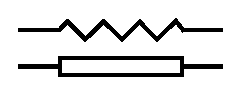
\includegraphics[scale=1.75]{grafiki/Resistors.eps} 
              \caption{Dwa stosowane symbole rezystorów,
              \\Źródło: \href{https://upload.wikimedia.org/wikipedia/commons/2/25/Resistors.svg}{Wikipedia}}
          \end{minipage}
        \end{figure}
      
      
        Jednostką rezystancji jest: \textit{Ohm} [$\Omega$]
        \begin{equation}
          1 \Omega = \frac{1 kg \cdot 1 m \textsuperscript{2}}{1 s \textsuperscript{3} \cdot 1 A \textsuperscript{2}} = \frac{1 V}{1 A}
        \end{equation}


      \subsubsection{Kondensator}
        Element elektroniczny bierny zbudowany z dwóch przewodników, inaczej okładek lub elektrod, rozdzielonych dielektrykiem. Przechowuje on energię w postaci pola elektrycznego.
        
        Doprowadzenie napięcia do okładek kondensatora powoduje zgromadzenie się na nich ładunku elektrycznego. Po odłączeniu od źródła napięcia, ładunki utrzymują się na okładkach siłami przyciągania elektrostatycznego.\textsuperscript{[2]}

        \begin{figure}[!ht]
            \begin{minipage}{.5\textwidth}
                \centering
                \includegraphics[scale=0.175]{grafiki/Kondensator_elektrolityczny_10F.png}
                \caption{Kondensator elektrolityczny $10F$,
                \\Źródło: \href{https://sklep.avt.pl/pol_pl_Kondensator-elektrolityczny-10F-2-5V-Samxon-DRE-172370_1.webp}{Link}}
            \end{minipage}
            \begin{minipage}{.5\textwidth}
                \centering
                \includegraphics[scale=0.075]{grafiki/Kondensator_symbol.jpg}
                \caption{Symbol służący do oznaczania kondensatorów w układach,
                \\Źródło: \href{https://elportal.pl/i/2022/05/06/9931-d309-1600x0_007-05.jpg}{Link}}
            \end{minipage}
        \end{figure}
        

        Jednostką pojemności jest: \textit{Farad} [$F$]
        \begin{equation}
          1 F = \frac{1C}{1V}
        \end{equation}

        %\addtolength{\footskip}{-1cm} % Zmienia pozycję linii w stopce
        \fancyfoot[L]{\textsuperscript{[1]}\url{https://pl.wikipedia.org/wiki/Rezystor}
        \\\textsuperscript{[2]}\url{https://pl.wikipedia.org/wiki/Kondensator}}
        \fancyfoot[C]{\thepage}
        \pagebreak
        \fancyfoot[L]{\textsuperscript{[3]}\url{https://pl.wikipedia.org/wiki/Cewka}}
        % \fancyfoot[L]{}

      \subsubsection{Cewka}
        Cewka to część obwodu elektrycznego, zaliczana do elementów biernych. Posiada uzwojenie, czyli zwoje przewodnika nawinięte na powierzchnię, na przykład walca czy pierścienia. Wytwarzają pole magnetyczne które, zgodnie z prawem Faradaya, może też wpłynąć na prąd elektryczny płynący w obwodzie.\textsuperscript{[3]}

        \begin{figure}[!ht]
          \begin{minipage}{.5\textwidth}
              \centering
              \includegraphics[scale=0.045]{grafiki/Cewka.png}
              \caption{Przykładowa cewka indukcyjna,
              \\Źródło: \href{https://pl.farnell.com/productimages/standard/pl_PL/2945407-40.jpg}{Link}}
          \end{minipage}
          \begin{minipage}{.5\textwidth}
              \centering
              \includegraphics[scale=0.085]{grafiki/Cewka_symbol.png}
              \caption{Symbol służący do oznaczania cewek w układach,
              \\Źródło: \href{https://fizyka.uniedu.pl/zwojnica/coil-146521/}{Link}}
          \end{minipage}
        \end{figure}

        Jednostka indukcyjności jest: \textit{Henr} [$H$]
        \begin{equation}
          1 H = \frac{1 V \cdot 1 s}{1 A}
        \end{equation}

    \subsection{Czwórnik}
      Nazywany również dwuwrotnikiem, to obwód elektryczny lub element obwodu, który posiada cztery zaciski, uporządkowane w dwie pary. Jedna z par stanowi wejście czwórnika, a druga wyjście.

      \begin{figure}[!ht]
            \centering
            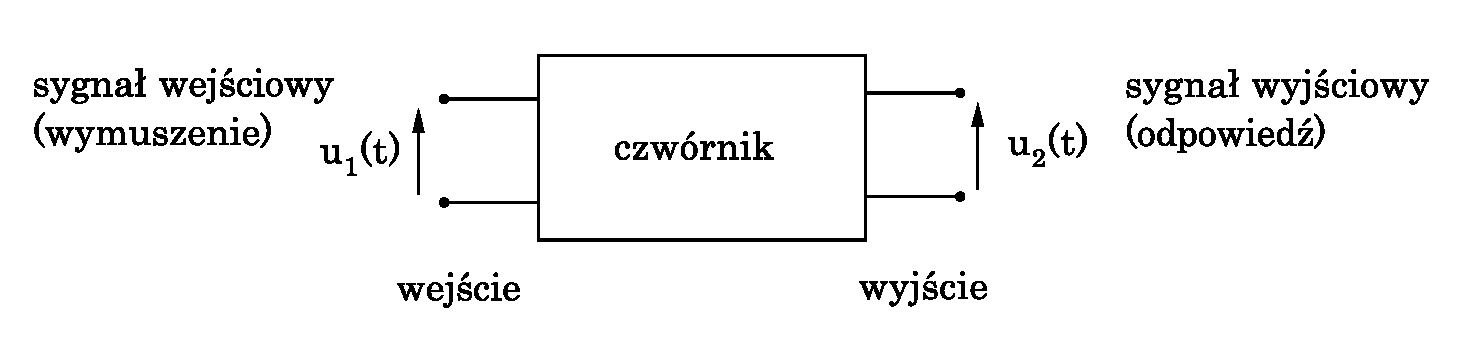
\includegraphics[scale=0.5]{grafiki/Czwornik.eps}
            \caption{Ogólny schemat działania czwórnika,
            \\Źródło: \href{https://spe.if.uj.edu.pl/literatura}{Strona wykładów}}
      \end{figure}

      Sprzężenie wyjścia z wejściem opisywane jest przez funkcję przejścia, nazywaną też \textbf{transmisją układu} lub \textbf{transmitancją}.

      \begin{equation}
        \textbf{T}  = \frac{u_2}{u_1}
        \label{eq2:transmisja}
      \end{equation}

    \subsection{Rodzaje czwórników}
      Możemy wyróżnić kilka rodzajów czwórników:
      \subsubsection{Wzmacniacze}
        Wzmacniacz to układ, który zwiększa moc sygnału wejściowego kosztem energii pobieranej ze źródła zasilającego.
      \subsubsection{Prostowniki}
        Element lub zestaw elementów elektronicznych służący do zamiany napięcia przemiennego na napięcie jednego znaku, które później może być zmienione na napięcie stałe.

        \pagebreak
        \fancyfoot[L]{}
      \subsubsection{Filtry}
        Filtr to układ elektroniczny, który przepuszcza sygnały sinusoidalne oraz składowe sygnałów o częstotliwościach powyżej pewnej określonej częstotliwości, a tłumi składowe leżące poniżej tej częstotliwości.
        
        Filtry możemy podzielić na:

          \paragraph{Górnoprzepustowe}
            \mbox{}\newline
            Inaczej znany jako \textit{Czwórnik CR} lub \textit{układ różniczkujący}. Filtr górnoprzepustowy przepuszcza składowe o częstotliwościach wyższych od częstotliwości granicznej, a tłumi składowe o częstotliwościach poniżej częstotliwości granicznej.

            Częstość graniczną oznaczamy jako:
            \begin{equation}
               \omega_0 = \frac{1}{CR} ,
            \end{equation}
            gdzie $CR$ to stała czasowa.

            Jak sama nazwa wskazuje układ ten można zbudować z kondensatora i opornika:

            \begin{figure}[!ht]
              \centering
              \begin{minipage}{.4\textwidth}
                \centering
                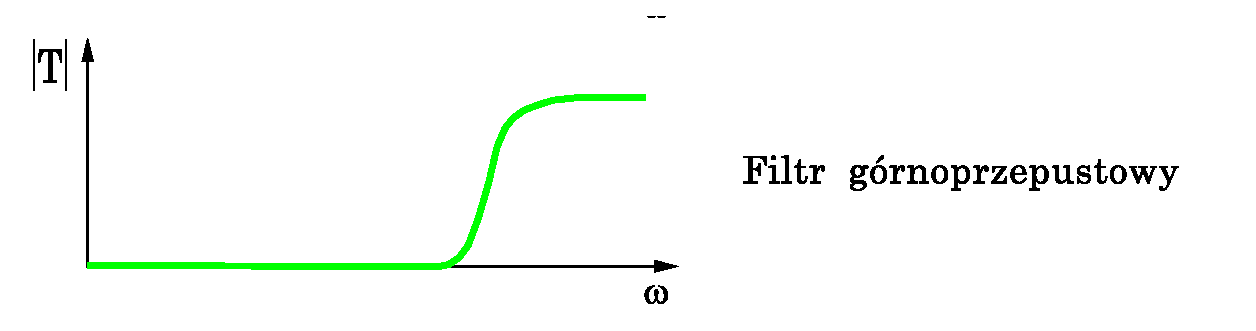
\includegraphics[scale=0.40]{grafiki/gornoprzepustowy.eps}
                \caption{Zależność funkcji przejścia $T$ od częstości w filtrze górnoprzepustowym, gdzie $|T(\omega)| = \sqrt{\frac{(\frac{\omega}{\omega_0})^2}{1+(\frac{\omega}{\omega_0})^2}}$,
                \\Źródło: \href{https://spe.if.uj.edu.pl/literatura}{Strona wykładów}}
                \label{fig1:gornoprzepustowy}
              \end{minipage}
              \begin{minipage}{.4\textwidth}
                \centering
                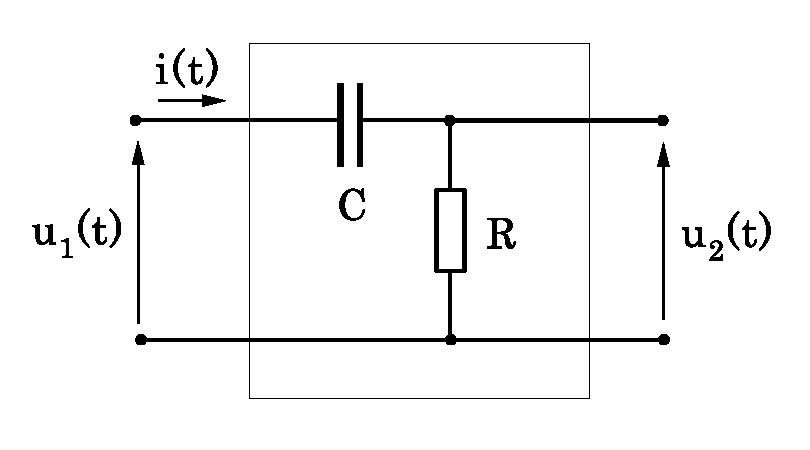
\includegraphics[scale=0.40]{grafiki/czwornik_CR.eps}
                \caption{Schemat budowy filtru górnoprzepustowego,
                \\Źródło: \href{https://spe.if.uj.edu.pl/literatura}{Strona wykładów}}
                \label{fig4:gornoprzepustowy_2}
              \end{minipage}
            \end{figure}

            Rysunek~\ref{fig1:gornoprzepustowy} przedstawia nic innego jak uproszczoną charakterystykę amplitudową tego filtru, czyli jak wpływa on na amplitudę sygnałów o różnych częstotliwościach.

            Natomiast jego charakterystyka fazowa prezentuje się nastepująco:
            \begin{figure}[!ht]
              \centering
              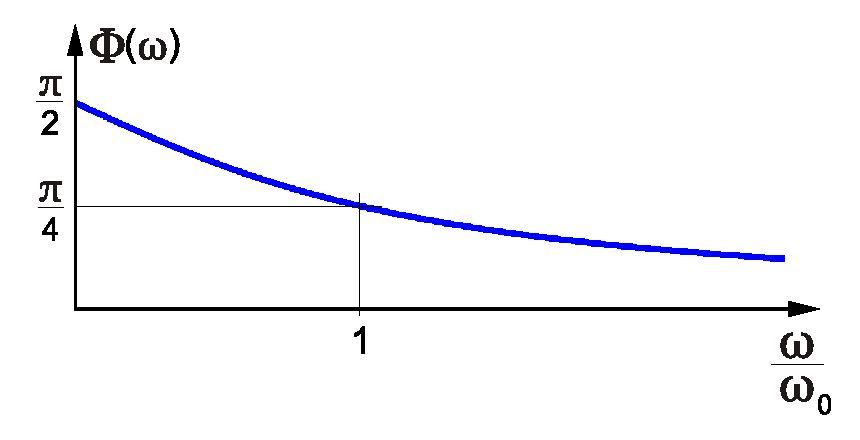
\includegraphics[scale=0.45]{grafiki/Cr_Phase.eps}
              \caption{Zależność przesunięcia fazy początkowej od ilorazu częstości granicznej i częstości w filtrze górnoprzepustowym, gdzie $\varPhi(\omega) = \arctan(\frac{\omega_0}{\omega})$,
              \\Źródło: \href{https://spe.if.uj.edu.pl/literatura}{Strona wykładów}}
            \end{figure}

          \paragraph{Środkowoprzepustowe}
            \mbox{}\newline
            Filtr środkowoprzepustowy przepuszcza składowe o częstotliwościach leżących w pobliżu częstotliwości granicznej, a tłumi składowe o częstotliwościach poniżej i powyżej częstotliwości granicznej.

            \begin{figure}[!ht]
              \centering
              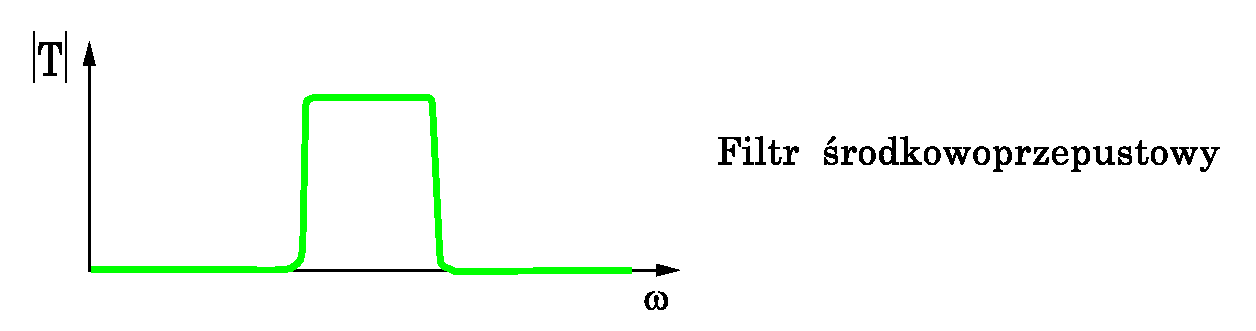
\includegraphics[scale=0.35]{grafiki/srodkowoprzepustowy.eps}
              \caption{Schemat działania filtru środkowoprzepustowego,
              \\Źródło: \href{https://spe.if.uj.edu.pl/literatura}{Strona wykładów}}
            \end{figure}

          \paragraph{Dolnoprzepustowe}
            \mbox{}\newline
            Inaczej znany jako \textit{Czwórnik RC} lub \textit{układ całkujący}. Filtr dolnoprzepustowy przepuszcza składowe o częstotliwościach niższych od częstotliwości granicznej, a tłumi składowe o częstotliwościach powyżej częstotliwości granicznej.
            Częstotliwość graniczna i stała czasowa jest identyczna jak w przypadku układu różniczkującego.

            Układ ten buduje się z jednego opornika oraz kondensatora:
            \begin{figure}[!ht]
              \centering
              \begin{minipage}{.4\textwidth}
                \centering
                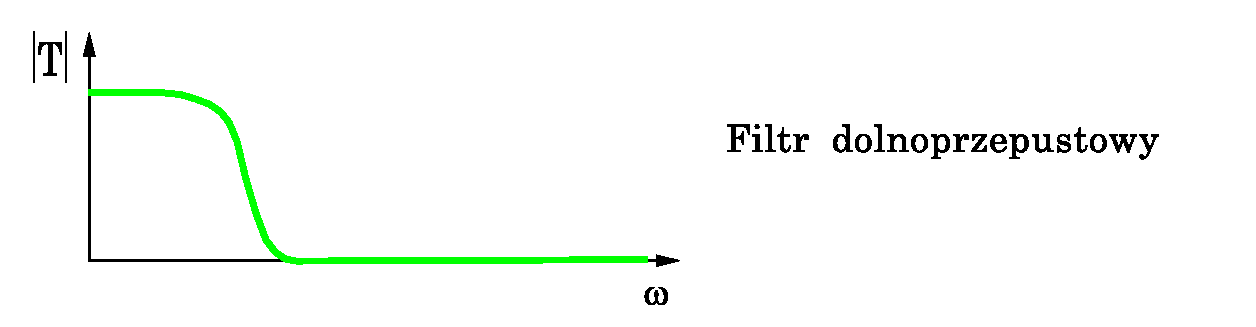
\includegraphics[scale=0.40]{grafiki/dolnoprzepustowy.eps}
                \caption{Zależność funkcji przejścia $T$ od częstości w filtrze dolnoprzepustowym, gdzie $|T(\omega)| = \sqrt{\frac{1}{1+(\frac{\omega}{\omega_0})^2}}$,
                \\Źródło: \href{https://spe.if.uj.edu.pl/literatura}{Strona wykładów}}
                \label{fig2:dolnoprzepustowy}
              \end{minipage}
              \begin{minipage}{.4\textwidth}
                \centering
                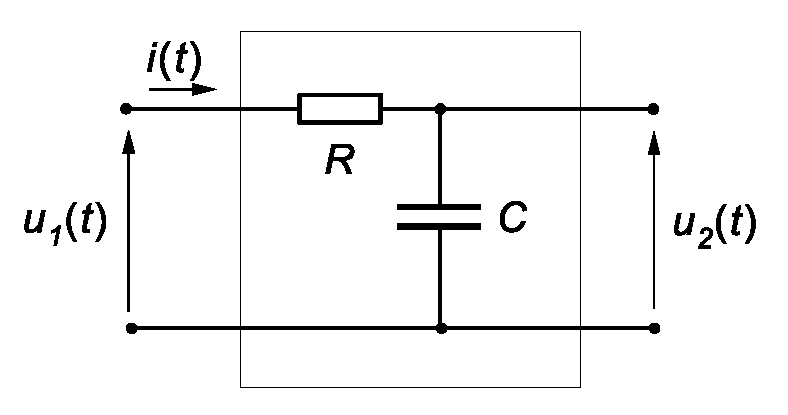
\includegraphics[scale=0.40]{grafiki/czwornik_RC.eps}
                \caption{Schemat budowy filtru dolnoprzepustowego,
                \\Źródło: \href{https://spe.if.uj.edu.pl/literatura}{Strona wykładów}}
                \label{fig3:dolnoprzepustowy_2}
              \end{minipage}
            \end{figure}

            Rysunek (\ref{fig2:dolnoprzepustowy}) prezentuje nam uproszczoną wersję charakterystyki amplitudowej a poniżej znajdziemy charakterystykę fazową tego układu:
            \begin{figure}[!ht]
              \centering
              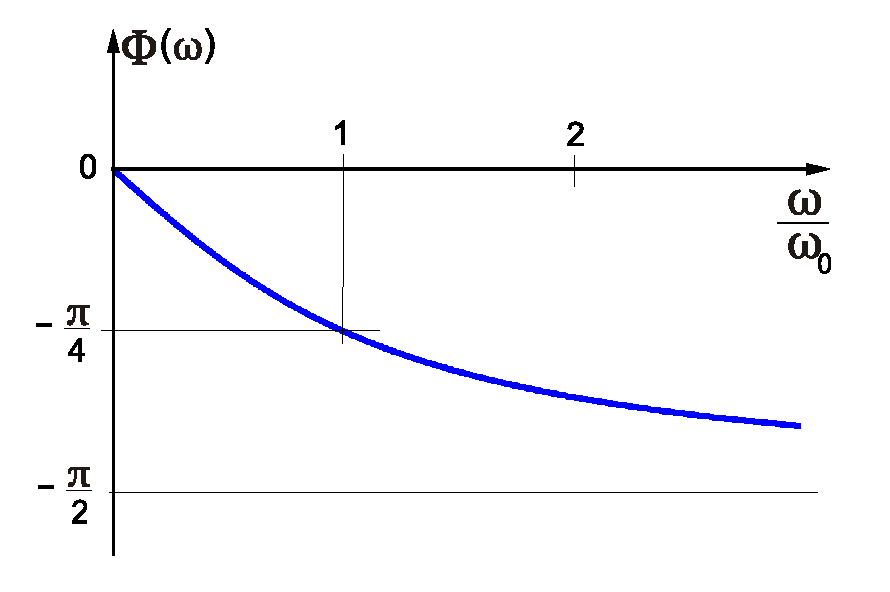
\includegraphics[scale=0.45]{grafiki/Rc_Phase.eps}
              \caption{Zależność przesunięcia fazy początkowej od ilorazu częstości i częstości granicznej w filtrze dolnoprzepustowym, gdzie $\varPhi(\omega) = -\arctan(\frac{\omega}{\omega_0})$,
              \\Źródło: \href{https://spe.if.uj.edu.pl/literatura}{Strona wykładów}}
            \end{figure}

          \paragraph{Środkowozaporowe}
            \mbox{}\newline
            Filtr środkowozaporowy tłumi składowe o częstotliwościach leżących w pobliżu częstotliwości granicznej, a przepuszcza składowe o częstotliwościach poniżej i powyżej częstotliwości granicznej.

            \begin{figure}[!ht]
              \centering
              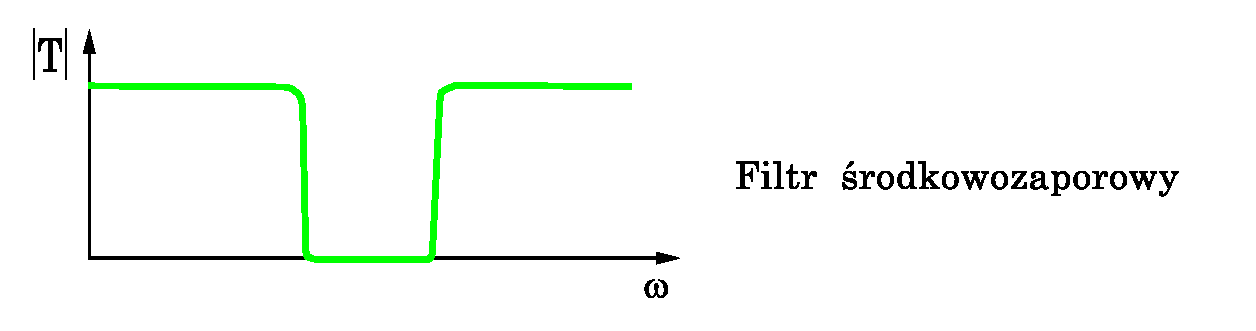
\includegraphics[scale=0.35]{grafiki/srodkowozaporowy.eps}
              \caption{Schemat działania filtru środkowozaporowego,
              \\Źródło: \href{https://spe.if.uj.edu.pl/literatura}{Strona wykładów}}
            \end{figure}

  \section{Ćwiczenia}
    \subsection{Ćwiczenie 2.1}
      Pierwszym zadaniem było zmontowanie układu różniczkującego, o stałej czasowej $\tau = RC$. Powinien on znajdować się w przedziale od $0.1 - 1 ms$. Układ miał zostać zmontowany na specjalnie przygotowanej płytce (numer 9) zawierającej podstawowowe elementy RLC.
      \subsubsection{Pomiary}
        Przy użyciu specjalnego miernika (oznaczonego numerem 1) uzyskałem poniższe pomiary:\\
        \mbox{} \qquad $R_1 = 5,58 k\Omega$ \\
        \mbox{} \qquad $R_2 = 2,981k\Omega$ \\
        \mbox{} \qquad $r = 47 \Omega$ \\
        \mbox{} \qquad $C = 141,7 nF$ \\
      \subsubsection{Stała czasowa}
        Do wykonania układu użyłem opornika $R_1$ oraz kondensatora $C$. Wykorzystując te dane do obliczenia stałej czasowej uzyskałem ponizszy wynik:
        \begin{equation}
          \begin{split}
            \tau &= R_1 \cdot C = 5,58k\Omega \cdot 141,7nF = 5,58 \cdot 141,7 \cdot 10^{-9+3} \Omega \cdot F = \\
            &= 790,686 \cdot 10^{-6} s = 0,000790686s = \mathbf{0,790686 ms}
          \end{split}
          \label{eq1:stala_czasowa_1}
        \end{equation}
        Jak możemy zobaczyć w równaniu (\ref{eq1:stala_czasowa_1}), wartość zawiera się w przewidzianym zakresie.

      \subsubsection{Układ CR}
        Kolejnym wymaganym krokiem było faktyczne zmontowanie układu różniczkującego, jak na schemacie (\ref{fig4:gornoprzepustowy_2}), w celu wykonania pomiarów.
          
        \begin{figure}[!ht]
          \centering
          \includegraphics[scale=0.1]{grafiki/uklad_CR_zdj.png}
          \caption{Poprawnie zmontowany układ CR,
              \\Źródło: Opracowanie własne}
        \end{figure}
        Do układu został również podłączony kabel prowadzący do oscyloskopu w celu wizualizacji sygnału. Nie wpływa to na wynik działania układu.
        
      \subsubsection{Pomiary dla 1V oraz 1kHz}
        Pierwszy pomiar z użyciem własnoręcznie zmontowanego układu dotyczył obliczenia transmisji układu (\ref{eq2:transmisja}), czyli stosunku amplitudy sygnału wyjściowego do amplitudy sygnału wejściowego, dla podanego na wejściu $1V$ oraz $1kHz$.

        \begin{equation}
          T = \frac{966mV}{984mV} = \frac{161}{164} \approx \mathbf{0.9817073}
        \end{equation}

        Natomiast przesunięcie fazy pomiędzy dwoma sygnałami wynosi:
        \begin{equation}
          \varphi = \mathbf{11.21^\circ}
        \end{equation}

        \begin{figure}[!ht]
          \centering
          \includegraphics[scale=0.5]{grafiki/1V_1kHz_sin_Overall_look.png}
          \caption{Uzyskany odczyt z oscyloskopu dla $1V$ oraz $1kHz$,
              \\Źródło: Opracowanie własne}
        \end{figure}

      \subsubsection{Uzyskana charakterystyka amplitudowa}
        W czasie zajęć zadaniem było zebranie danych z różnych zakresów częstotliwości w celu utworzenia wykresu.

        \begin{table}[h]
          \centering
          \scalebox{0.65}{
          \begin{tabular}{|c|c|c|c|c|}
          \hline
          \textbf{Hz} & \textbf{Amplituda wyjściowa[mV]} & \textbf{Amplituda wejściowa[mV]} & \textbf{Stosunek Amplitud(wyjściowa/wejściowa)} & \textbf{Krzywa teoretyczna} \\
          \hline
          100 & 433 &	985 &	0,439593909	& 0,331910059 \\
          200 & 696 &	984 &	0,707317073	& 0,498397106 \\
          300 & 806 &	984 &	0,819105691	& 0,598460234 \\
          400 & 880 &	984 &	0,894308943	& 0,665240347 \\
          500 & 912 &	984 &	0,926829268	& 0,712975429 \\
          600 & 928 &	984 &	0,943089431	& 0,748795899 \\
          700 & 936 &	984 &	0,951219512	& 0,776667627 \\
          800 & 947 &	984 &	0,962398374	& 0,798972171 \\
          900 & 955 &	984 &	0,970528455	& 0,81722608 \\
          1 000 &	968 &	984 &	0,983739837	& 0,832440929 \\
          2 000 &	976 &	984 &	0,991869919	& 0,908559633 \\
          3 000 &	976 &	984 &	0,991869919	& 0,937123265 \\
          4 000 &	976 &	984 &	0,991869919	& 0,952089332 \\
          5 000 &	976 &	984 &	0,991869919	& 0,961300643 \\
          6 000 &	976 &	984 &	0,991869919	& 0,96754118 \\
          7 000 &	976 &	984 &	0,991869919	& 0,972048544 \\
          8 000 &	976 &	984 &	0,991869919	& 0,975456724 \\
          9 000 &	976 &	984 &	0,991869919	& 0,978124098 \\
          10 000 & 984 &	984 &	1 &	0,980268524 \\
         
          \hline
          \end{tabular}}
          \caption{Dane użyte do stworzenia wykresu,
          \\Źródło: Opracowanie własne}
          \label{Tabela1}
        \end{table}

        Stosunek amplitud jest to po prostu iloraz amplitudy wejściowej do wyjściowej. Krzywa teoretyczna została obliczona przy użyciu wzoru:
        \begin{equation}
          |T(\omega)| = \sqrt{\frac{(\frac{\omega}{\omega_0})^2}{1+(\frac{\omega}{\omega_0})^2}}
        \end{equation}

        \pagebreak

        \begin{figure}[!ht]
          \centering
          \includegraphics[scale=0.75]{grafiki/1_amp_plot.eps}
          \caption{Uzyskany wynik porównany z krzywą teoretyczną,
              \\Źródło: Opracowanie własne}
        \end{figure}

       Linia fioletowa to różnica amplitud uzyskana przy pomocy pomiarów własnych. Jest ona również wzbogacona o odchylenie standardowe reprezentowane poprzez zakres zaznaczony w każdym punkcie. Linia przerywana natomiast to wartość idealna wyliczona ze wzoru opierającego się na częstotliwości granicznej.

       Same obliczenie częstotliwości granicznej przezentuje się nastepująco:
       \begin{equation}
        f_0 = \frac{\omega_0}{2\pi} = \frac{1}{2\pi} \cdot \frac{1}{RC} = \frac{1}{2 \pi RC} = \frac{1}{2 \cdot \pi \cdot 0,790686} = \mathbf{201,287 Hz}
       \end{equation}

      \subsubsection{Uzyskana charakterystyka fazowa}
        W charakterystyce fazowej ukazujemy natomiast przesunięcie sygnału w czasie, spowodowane przez dłuższą drogę prowadzącą przez układ.
        
        \begin{table}[!ht]
          \begin{minipage}{.4\textwidth}
            \centering
            \scalebox{0.65}{
            \begin{tabular}{|c|c|}
            \hline
            \textbf{Hz} & \textbf{Faza[stopnie]} \\
            \hline
            100 & 68.53 \\
            200 & 45.25 \\
            300 & 32.54 \\
            400 & 25.46 \\
            500 & 22.32 \\
            600 & 15.97 \\
            700 & 16.23 \\
            800 & 14.21 \\
            900 & 12.98 \\
            1000 & 10.22 \\
            2000 & 6.339 \\
            3000 & 2.921 \\
            4000 & 1.302 \\

            \hline
            \end{tabular}}
            \caption{Dane odczytane z oscyloskopu,
            \\Źródło: Opracowanie własne}
            \label{Tabela2}
          \end{minipage}%
          \begin{minipage}{.4\textwidth}
            \centering
            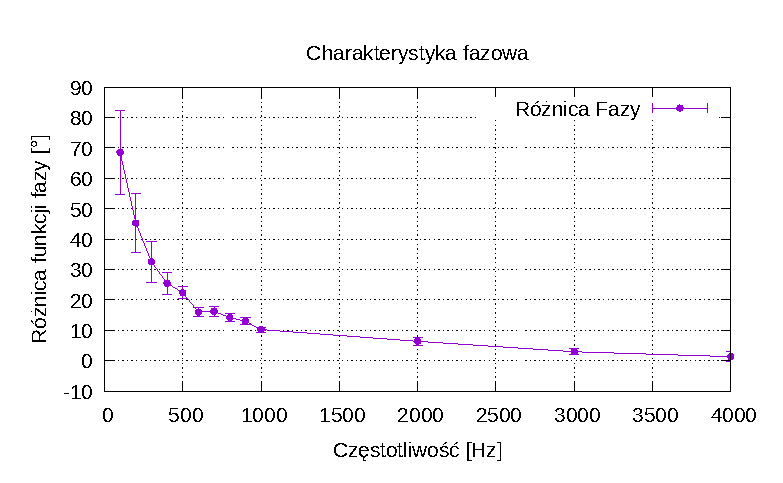
\includegraphics[scale=0.75]{grafiki/1_phase_plot.eps}
            \captionof{figure}{Wykres zależności kąta fazowego $\theta$ od częstotliwości,
                \\Źródło: Opracowanie własne}
          \end{minipage}
        \end{table}
        
        dla $f_0 = 201,287 Hz$ kąt $\theta$ będzie wahał się wokół $45^\circ$.

    \subsection{Ćwiczenie 2.2}
      Ćwiczenie to polegało na porównaniu zachowania fal prostokątnej oraz trójkątnej dla różnych okresów:\\ \\
      $T_{mniejsze}= 0,1 \cdot \tau = 0,079068 ms$ \\
      $T_{rowne} = 1 \cdot \tau = 0,79068 ms$ \\
      $T_{wieksze} = 10 \cdot \tau = 7,9068 ms$
     
      \subsubsection{Fala Prostokątna}
        \begin{figure}[!ht]
          \centering
          \begin{minipage}{.4\textwidth}
            \centering
            \includegraphics[scale=0.25]{grafiki/P_T_mniejszy.png}
            \caption{Impulsy prostokątne o okresie T \textbf{\textcolor{red}{mniejszym}} od stałej czasowej $\tau$,
              \\Źródło: Opracowanie własne}
          \end{minipage}
          \begin{minipage}{.4\textwidth}
            \centering
            \includegraphics[scale=0.25]{grafiki/P_T_wiekszy.png}
            \caption{Impulsy prostokątne o okresie T \textbf{\textcolor{green}{większym}} od stałej czasowej $\tau$,
            \\Źródło: Opracowanie własne}
          \end{minipage}
        \end{figure}

        \begin{figure}[!ht]
          \centering
          \includegraphics[scale=0.2]{grafiki/P_T.png}
          \caption{Impulsy prostokątne o okresie T \textbf{\textcolor{yellow}{równym}} stałej czasowej $\tau$,
              \\Źródło: Opracowanie własne}
        \end{figure}

      \subsubsection{Fala Trójkątna}

        \begin{figure}[!ht]
          \centering
          \begin{minipage}{.4\textwidth}
            \centering
            \includegraphics[scale=0.25]{grafiki/T_T_mniejszy.png}
            \caption{Impulsy trójkątne o okresie T \textbf{\textcolor{red}{mniejszym}} od stałej czasowej $\tau$,
              \\Źródło: Opracowanie własne}
          \end{minipage}
          \begin{minipage}{.4\textwidth}
            \centering
            \includegraphics[scale=0.25]{grafiki/T_T_wiekszy.png}
            \caption{Impulsy trójkątne o okresie T \textbf{\textcolor{green}{większym}} od stałej czasowej $\tau$,
            \\Źródło: Opracowanie własne}
          \end{minipage}
        \end{figure}
        \begin{figure}[!ht]
          \centering
          \includegraphics[scale=0.25]{grafiki/T_T.png}
          \caption{Impulsy trójkątne o okresie T \textbf{\textcolor{yellow}{równym}} stałej czasowej $\tau$,
              \\Źródło: Opracowanie własne}
        \end{figure}

        Jak jesteśmy w stanie zaobserwować, w obu przypadkach, zmiany zachodzą w przykładzie gdzie T jest większe -- co za tym idzie, \textbf{układ różniczkuje lepiej sygnały o niższych częstotliwościach}.
        \pagebreak
    \subsection{Ćwiczenie 2.3}
      Kolejnym punktem zadań było przekonstruowanie istniejącego układu w układ całkujący według rysunku (\ref{fig3:dolnoprzepustowy_2}).

      \subsubsection{Układ RC}
        \begin{figure}[!ht]
          \centering
          \includegraphics[scale=0.12]{grafiki/uklad_RC_zdj.png}
          \caption{Poprawnie zmontowany układ RC,
              \\Źródło: Opracowanie własne} 
        \end{figure}

      \subsubsection{Pomiary dla 1V oraz 1kHz}
        Stosunek amplitudy sygnału wyjściowego do amplitudy sygnału wejściowego,w tym przypadku dla $1V$ oraz $1kHz$: wynosi:

        \begin{equation}
          T = \frac{218mV}{976mV} = \frac{109}{488} \approx \mathbf{0.2233606}
        \end{equation}

        Przesunięcie fazy pomiędzy dwoma sygnałami wynosi średnio:
        \begin{equation}
          \varphi = \mathbf{-32,11^\circ}
        \end{equation}

        \begin{figure}[!ht]
          \centering
          \includegraphics[scale=0.45]{grafiki/1kHz.png}
          \caption{Uzyskany odczyt z oscyloskopu dla $1V$ oraz $1kHz$,
              \\Źródło: Opracowanie własne}
        \end{figure}
        \pagebreak

      \subsubsection{Charakterystyka amplitudowa}

        \begin{table}[h]
          \centering
          \scalebox{0.65}{
          \begin{tabular}{|c|c|c|c|c|}
          \hline
          \textbf{Hz} & \textbf{Amplituda wyjściowa[mV]} & \textbf{Amplituda wejściowa[mV]} & \textbf{Stosunek Amplitud(wyjściowa/wejściowa)} & \textbf{Krzywa teoretyczna} \\
          \hline
          100 & 888 & 984 & 0.902439024 & 0.66809074 \\
          200 & 680 & 984 & 0.691056911 & 0.501603795 \\
          300 & 536 & 984 & 0.544715447 & 0.401540632 \\
          400 & 424 & 984 & 0.430894309 & 0.334760455 \\
          500 & 360 & 984 & 0.365853659 & 0.287025308 \\
          600 & 304 & 984 & 0.308943089 & 0.251204778 \\
          700 & 256 & 984 & 0.260162602 & 0.223332998 \\
          800 & 280 & 984 & 0.284552846 & 0.201028408 \\
          900 & 200 & 984 & 0.203252033 & 0.182774458 \\
          1000 & 248 & 984 & 0.25203252 & 0.167559573 \\
          2000 & 94 & 984 & 0.095528455 & 0.091440666 \\
          3000 & 64 & 984 & 0.06504065 & 0.062876947 \\
          4000 & 60 & 984 & 0.06097561 & 0.047910832 \\
          5000 & 36.8 & 984 & 0.037398374 & 0.038699491 \\
          6000 & 31.2 & 984 & 0.031707317 & 0.032458933 \\
          7000 & 37.2 & 984 & 0.037804878 & 0.027951554 \\
          8000 & 23.6 & 984 & 0.02398374 & 0.024543363 \\
          9000 & 20.4 & 984 & 0.020731707 & 0.021875979 \\
          10000 & 17.2 & 984 & 0.017479675 & 0.019731546 \\
          20000 & 7.2 & 984 & 0.007317073 & 0.009964076 \\
          \hline
          \end{tabular}}
          \caption{Dane użyte do stworzenia wykresu,
          \\Źródło: Opracowanie własne}
          \label{Tabela3}
        \end{table}

        Stosunek amplitud jest to po prostu iloraz amplitudy wejściowej do wyjściowej. Krzywa teoretyczna została obliczona przy użyciu wzoru:
        \begin{equation}
          |T(\omega)| = \sqrt{\frac{1}{1+(\frac{\omega}{\omega_0})^2}}
        \end{equation}

      \begin{figure}[!ht]
        \centering
        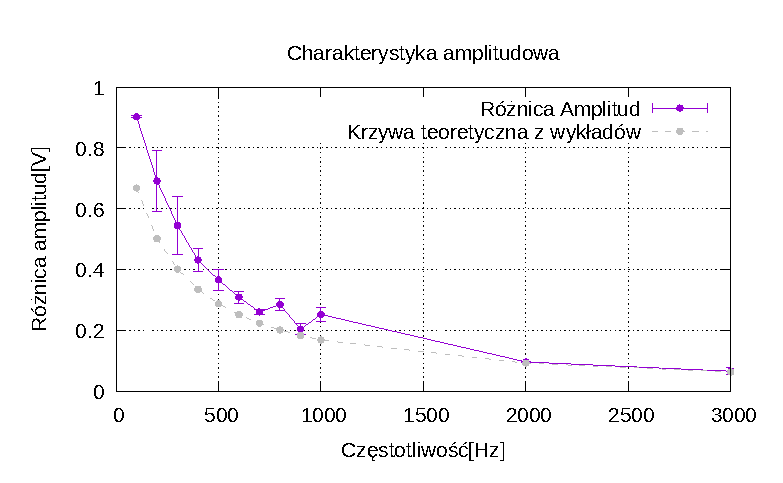
\includegraphics[scale=0.75]{grafiki/2_amp_plot.eps}
        \caption{Uzyskany wynik porównany z krzywą teoretyczną,
            \\Źródło: Opracowanie własne}
      \end{figure}

      Jak widzimy odczyty z oscyloskopu pokrywają się z krzywą teoretyczną jeśli chodzi o ogólny kształt wykresu.
      \pagebreak

      \subsubsection{Charakterystyka fazowa}

      \begin{table}[!ht]
        \begin{minipage}{.4\textwidth}
          \centering
          \scalebox{0.65}{
          \begin{tabular}{|c|c|}
          \hline
          \textbf{Hz} & \textbf{Faza[stopnie]} \\
          \hline
          100 &	-26,61 \\
          200 &	-42,48 \\
          300 &	-56,33 \\
          400 &	-60,65 \\
          500 &	-66,51 \\
          600 &	-69,42 \\
          700 &	-67,04 \\
          800 &	-71,64 \\
          900 &	-76,1 \\
          1 000 &	-78,96 \\
          2 000 &	-82,64 \\
          3 000 &	-80,58 \\
          4 000 &	-76,69 \\
          5 000 &	-84,27 \\
          6 000 &	-84,47 \\
          7 000 &	-82,75 \\
          8 000 &	-158,6 \\
          9 000 &	-76,32 \\
          10 000 &	-131,9 \\ 
          \hline
          \end{tabular}}
          \caption{Dane odczytane z oscyloskopu,
          \\Źródło: Opracowanie własne}
          \label{Tabela4}
        \end{minipage}
        \begin{minipage}{.4\textwidth}
          \centering
          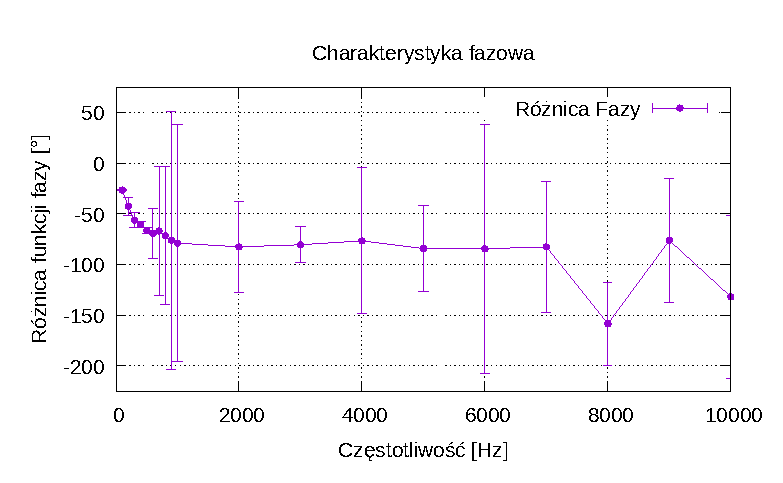
\includegraphics[scale=0.75]{grafiki/2_phase_plot.eps}
          \captionof{figure}{Wykres zależności kąta fazowego $\theta$ od częstotliwości,
              \\Źródło: Opracowanie własne}
        \end{minipage}
      \end{table}

      Charakterystyka fazowa ukazująca przesunięcie sygnału w czasie, również przyjmuje oczekiwany kształt jednak powyżej $7kHz$ momentu występują pewne zakłocenia sygnału.

    \subsubsection{Przebieg impulsów wyjściowych i wejściowych dla fali prostokątnej}
      W tej części polecenia zadaniem było zaobserwować powstawanie charakterystycznego czasu narastania dla sygnału o fali prostokątnej w miarę stopniowej zmiany okresu zaczynając od wielkości  $T = 0,5 \cdot \tau$ aż do $T = 10 \cdot \tau$.

      \begin{figure}[!ht]
        \centering
        \begin{minipage}{.4\textwidth}
          \centering
          \includegraphics[scale=0.25]{grafiki/0.5t.png}
          \caption{Impulsy prostokątne o okresie $T = 0.5 \tau$,
            \\Źródło: Opracowanie własne}
        \end{minipage}
        \begin{minipage}{.4\textwidth}
          \centering
          \includegraphics[scale=0.25]{grafiki/5t.png}
          \caption{Impulsy prostokątne o okresie $T = 5 \tau$,
          \\Źródło: Opracowanie własne}
          \label{fig5:impuls5T}
        \end{minipage}
      \end{figure}
      \begin{figure}[!ht]
        \centering
        \includegraphics[scale=0.25]{grafiki/10t.png}
        \caption{Impulsy prostokątne o okresie $T = 10 \tau$,
            \\Źródło: Opracowanie własne}
      \end{figure}

      \pagebreak

      \begin{itemize}
        \item Jak jesteśmy wstanie zaobserwować dla $T = 0.5 \tau$ sygnał charakterystyką przypomina bardziej falę trójkątną, impulsy wejściowe przyjmują postać funkcji liniowej.
        \item Dla okresu równego 5 $\tau$ zaczynamy zauważać powolną zmianę natury czasu narastania, przypominają ona w tych fragmentach parabolę.
        \item Finalnie przy okresie rzędu 10 $\tau$ otrzymujemy oczekiwany efekt, czyli charakterystyczny kształt zaczynający się gwałtownym implusem na początku oraz powolnym wejściem na docelową amplitudę idealnie na końcu sygnału prostokątnego.
      \end{itemize}
      Dla $5 \tau$ okres układu wynosi:
      \begin{equation}
        T = 5 \tau = 5 \cdot 0.790686ms = \mathbf{3.95343ms} 
      \end{equation}
      Z rysunku (\ref{fig5:impuls5T}) dzięki ustawionemu measurement'owi jesteśmy wstanie odczytać w prosty sposób \textbf{czas narastania} który wynosi \textbf{średnio 1,562ms}.


  \section{Omówienie wyników}
    \subsection{Ćwiczenie 2.1}
      Po przeprowadzeniu pomiarów rezystancji ($R$) i pojemności ($C$), obliczono stałą czasową układu. Wynosiła ona $0.790686$ ms, co mieściło się w zakładanym przedziale $0.1 - 1$ ms.
      Przeprowadzony został pomiar transmisji układu oraz przesunięcia fazowego dla sygnału wejściowego o amplitudzie $1V$ i częstotliwości $1kHz$. Stosunek amplitud wynosił około $0.9817073$, a przesunięcie fazowe wynosiło $11.21^\circ$. Otrzymane wartości są jak najbardziej wiarygodne oraz potwierdzają poprawność działania układu różniczkującego.

      Analizując uzyskaną charakterystykę amplitudową jesteśmy wstanie zauważyć podobny profil krzywej do tej uzyskanej teoretycznym wzorem. Mimo wszystko widoczne jest ewidentne przesunięcie wykresu o $\approx 0,1V$ od idealnych wartości. Została ona stworzona przy zastosowaniu wzoru:
      \begin{equation}
        |T(\omega)| = \sqrt{\frac{(\frac{\omega}{\omega_0})^2}{1+(\frac{\omega}{\omega_0})^2}}
      \end{equation}

      Co ciekawe jeśli popatrzymy na uzyskany wynik przy obliczaniu częstotliwości granicznej to z wykresu wynika, że odpowiada on wartości $\approx 0,71$ czyli $\frac{1}{\sqrt{2}}$ co wynika bezpośrednio z powyższego wzoru. Krzywa ta jest w takim razie poprawnie wykonana.

      Wykres zmiany przesunięcia fazy również odpowiada kształtem oczekiwanej funkcji. Sam odczyt kąta $\theta$ jest również poprawny ponieważ:
      \begin{equation}
        arctg(45^\circ) \approx 0,6665773
      \end{equation}
      Co jest wystarczająco blisko wartości przyjmowanej przez $\frac{\pi}{4}$ biorąc pod uwagę odchylenie wyniku.

    \subsection{Ćwiczenie 2.2}
      W powyższym zadaniu wykonano porównianie zachowania fal prostokątnej i trójkątnej dla różnych okresów, które były większe lub mniejsze od stałej czasowej $\tau$.

      Zaobserwować można było, że dla okresów większych od $\tau$, sygnał był różniczkowalny tak w przeciwieństwie do mniejszych okresów gdzie przypominały one funkcję wejściową.
    
      Wnioskiem z tego eksperymentu jest to, że układ różniczkujący lepiej radzi sobie z sygnałami o niższych częstotliwościach. Natomiast dla sygnałów o wyższych częstotliwościach, zachowanie układu różniczkującego może być mniej skuteczne, szczególnie gdy okres jest mniejszy od $\tau$.

    \subsection{Ćwiczenie 2.3}
      W tym podpunkcie zostały wykonane bliźniacze badania co w zadaniu $2.1$. Obliczony został stosunek amplitudy sygnału wyjściowego do wejściowego oraz przesunięcie fazowe dla parametrów $1V$ oraz $1kHz$ co pozwoliło określić wzmocnienie układu dla tej konkretnej częstotliwości i napięcia.

      Wyniki dotyczące charakterystyki amplitudowej i fazowej prezentują się bardzo podobnie. Oba pokrywają się ogólnym kształtem funkcji aczkolwiek w przypadku różnicy amplitud dalej występuje lekkie przesunięcie danych. Natomiast wykreślona funkcja fazy powyżej częstotliwości $7kHz$ ukazuje lekko odbiegające wartości zapewne przez występujące zakłócenia i wstarczająco słaby już sygnał. Zapisanie tak wysokich wartości wynika tylko z mojego kurczowego trzymania się instrukcji oraz chęci ukazania co może się wydarzyć gdy sygnał wystarczająco osłabnie.

      Punkt dotyczący badania impulsów wejściowych i wyjściowych przebiegł pomyślnie oraz dostarczył pożądanych wyników. Dziesięciokrotność $\tau$ prezentuje oczekiwane impulsy wejściowe i wyjściowe. Obliczone wartości teoretyczne czasu narasatania zgadzają się z odczytanymi pomiarami: \\
      $\frac{0,5 \cdot \tau}{2}  = \frac{0,395343 ms}{2} = 0,1976715 ms \sim \mathbf{0,2ms}$ (Odczytane z oscyloskopu) \\
      $\frac{5 \cdot \tau}{2}  = \frac{3,95343 ms}{2} = 1,976715 ms \sim \mathbf{2ms}$ (Odczytane z oscyloskopu) \\
      $\frac{10 \cdot \tau}{2}  = \frac{7,90686 ms}{2} = 3,95343 ms \sim \mathbf{4ms}$ (Odczytane z oscyloskopu) \\

      Reszta wykonanych screenshot'ów znajduje się w notatkach i materiałach z zajęć.



  \section{Podsumowanie}
    Drugie ćwiczenia laboratoryjne dostarczyły cennej wiedzy na temat podstawowych elementów elektronicznych, jak również ich zastosowań w praktyce. Podczas laboratorium udało się zbudować układy różniczkujące, całkujące oraz zbadać ich charakterystyki amplitudowe i fazowe. Dodatkowo, porównano zachowanie fal prostokątnych i trójkątnych dla różnych okresów, co pozwoliło lepiej zrozumieć działanie tych układów. Całość doświadczenia była świetnym sposobem na lepsze zrozumienie teoretycznych podstaw elektroniki oraz nauczenie się praktycznych umiejętności związanych z montażem i pomiarami na układach elektronicznych.

  \section{Notatki i materiały z zajęć}
    \begin{figure}[!ht]
      \centering
      \begin{minipage}{.4\textwidth}
        \centering
        \includegraphics[scale=0.15]{grafiki/notatki_3.jpg}
        \caption{Wypełniona karta pracy,
          \\Źródło: Opracowanie własne}
      \end{minipage}
      \begin{minipage}{.4\textwidth}
        \centering
        \includegraphics[scale=0.15]{grafiki/notatki_2.jpg}
        \caption{Wypełniona karta pracy,
        \\Źródło: Opracowanie własne}
      \end{minipage}
    \end{figure}

    \begin{figure}[!ht]
      \centering
      \begin{minipage}{.4\textwidth}
        \centering
        \includegraphics[scale=0.15]{grafiki/notatki_1.jpg}
        \caption{Wypełniona karta pracy,
          \\Źródło: Opracowanie własne}
      \end{minipage}
      \begin{minipage}{.4\textwidth}
        \centering
        \includegraphics[scale=0.3]{grafiki/1t.png}
        \caption{Impulsy prostokątne o okresie $T = 1 \tau$,
        \\Źródło: Opracowanie własne}
      \end{minipage}
    \end{figure}

    \begin{figure}[!ht]
      \centering
      \begin{minipage}{.4\textwidth}
        \centering
        \includegraphics[scale=0.3]{grafiki/2t.png}
        \caption{Impulsy prostokątne o okresie $T = 2 \tau$,
          \\Źródło: Opracowanie własne}
      \end{minipage}
      \begin{minipage}{.4\textwidth}
        \centering
        \includegraphics[scale=0.3]{grafiki/3t.png}
        \caption{Impulsy prostokątne o okresie $T = 3 \tau$,
        \\Źródło: Opracowanie własne}
      \end{minipage}
    \end{figure}

    \begin{figure}[!ht]
      \centering
      \begin{minipage}{.4\textwidth}
        \centering
        \includegraphics[scale=0.3]{grafiki/4t.png}
        \caption{Impulsy prostokątne o okresie $T = 4 \tau$,
          \\Źródło: Opracowanie własne}
      \end{minipage}
      \begin{minipage}{.4\textwidth}
        \centering
        \includegraphics[scale=0.3]{grafiki/6t.png}
        \caption{Impulsy prostokątne o okresie $T = 6 \tau$,
        \\Źródło: Opracowanie własne}
      \end{minipage}
    \end{figure}

    \begin{figure}[!ht]
      \centering
      \begin{minipage}{.4\textwidth}
        \centering
        \includegraphics[scale=0.3]{grafiki/7t.png}
        \caption{Impulsy prostokątne o okresie $T = 7 \tau$,
          \\Źródło: Opracowanie własne}
      \end{minipage}
      \begin{minipage}{.4\textwidth}
        \centering
        \includegraphics[scale=0.3]{grafiki/8t.png}
        \caption{Impulsy prostokątne o okresie $T = 8 \tau$,
        \\Źródło: Opracowanie własne}
      \end{minipage}
    \end{figure}

    \begin{figure}[!ht]
      \centering
      \begin{minipage}{.4\textwidth}
        \centering
        \includegraphics[scale=0.3]{grafiki/8t.png}
        \caption{Impulsy prostokątne o okresie $T = 8 \tau$,
          \\Źródło: Opracowanie własne}
      \end{minipage}
      \begin{minipage}{.4\textwidth}
        \centering
        \includegraphics[scale=0.23]{grafiki/9t.png}
        \caption{Impulsy prostokątne o okresie $T = 9 \tau$,
        \\Źródło: Opracowanie własne}
      \end{minipage}
    \end{figure}
\end{document}